% These packages are optional, depending whether you want the features they provide.
% See the LaTeX Companion or other references for full information.
% !TEX TS-program = pdflatex
% !TEX encoding = UTF-8 Unicode

% This is a simple template for a LaTeX document using the "article" class.
% See "book", "report", "letter" for other types of document.

\documentclass[12pt]{article} % use larger type; default would be 10pt
\usepackage[T2A]{fontenc}
\usepackage[utf8]{inputenc} % set input encoding (not needed with XeLaTeX)
\usepackage[russian]{babel}
%%% Examples of Article customizations
% These packages are optional, depending whether you want the features they provide.
% See the LaTeX Companion or other references for full information.

%%% PAGE DIMENSIONS
\usepackage{geometry}

\usepackage{fancyhdr} 
\geometry{a4paper} % or letterpaper (US) or a5paper or....
% \geometry{margin=2in} % for example, change the margins to 2 inches all round
% \geometry{landscape} % set up the page for landscape
%   read geometry.pdf for detailed page layout information
\usepackage{sectsty}
\usepackage{graphicx} % support the \includegraphics command and options
\usepackage{mathtext}
\usepackage{amsmath}
\usepackage{amsfonts}
% \usepackage[indentfill]{indentskip} % Activate to begin indentagraphs with an empty line rather than an indent
\usepackage{biblatex}
\usepackage{hyperref}
\hypersetup{
  colorlinks=true,
  linkcolor=blue,
  urlcolor=green
}
%%% END Article customizations

%%% The "real" document content comes below...
\usepackage{setspace}
\usepackage[section]{minted}

%%% ToC (table of contents) APPEARANCE
\usepackage[nottoc,notlof,notlot]{tocbibind} % Put the bibliography in the ToC
\usepackage[titles,subfigure]{tocloft} % Alter the style of the Table of Contents

%\date{} % Activate to display a given date or no date (if empty),
         % otherwise the current date is printed 
\usepackage{physics}
\usepackage{float}
\begin{titlepage}
	\thispagestyle{empty}
	\begin{center}
	\large{МИНОБРНАУКИ РОССИИ}\\
	\footnotesize{ФЕДЕРАЛЬНОЕ ГОСУДАРСТВЕННОЕ БЮДЖЕТНОE ОБРАЗОВАТЕЛЬНОЕ УЧРЕЖДЕНИЕ}\\ 
	\footnotesize{ВЫСШЕГО ПРОФЕССИОНАЛЬНОГО ОБРАЗОВАНИЯ}\\ 
	\small{\textbf{«САНКТ-ПЕТЕРБУРГСКИЙ ГОСУДАРСТВЕННЫЙ ПОЛИТЕХНИЧЕСКИЙ УНИВЕРСИТЕТ ПЕТРА ВЕЛИКОГО»}}\\
	\hfill \break
	\normalsize{Институт компьютерных наук и технологий}\\
	\hfill \break
	\normalsize{Высшая школа искусственного интеллекта}\\
	\hfill\break
	\begin{center}
		\normalsize{Дисциплина: \\ПРОГРАММИРОВАНИЕ МИКРОКОНТРОЛЛЕРОВ}
	\end{center}
	\hfill \break
	\hfill \break
	\large{ОТЧЕТ}\\
	\large{По лабораторной работе №5}\\
	\medium{Тема: ЦАП и волна}\\
	\hfill \break
	\hfill \break
	\hfill \break
	\hfill \break
	\hfill \break
	\hfill \break
\end{center}	

\normalsize{ 
	\begin{tabular}{ccc}
		Обучающийся &  гр. 3530201/10001 & Нгуен Куок Дат \\\\
		Руководитель & \hrulefill 				&Вербова Наталья Михайловна\\\\
	\end{tabular}
}\\
\hfill \break
\hfill \break
\hfill \break
\hfill \break
\begin{center} Санкт-Петербург 2022 
\end{center}
\end{titlepage}
\usepackage{indentfirst}

\begin{document}
\begin{center}
\input{titlepage}
\end{center}
\doublespacing
\tableofcontents
\newpage
\section{Цель и постановка задачи}
\subsection{Цель работы}
Ознакомится с архитектурой низкоуровневых библиотек и промежуточного программного обеспечения микроконтроллера. Закрепить навыки работы с осциллографом и оценочной платой MCBSTM32F200 в качестве измерительного генератора.

\subsection{Постановка задачи}
Разработать программу для микроконтроллера (МК) STM32F200, которая:\\

\begin{itemize}
\item выдает на выходе ЦАП заданный уровень напряжения.
\item генерирует на выходе ЦАП микроконтроллера (МК) STM32F200 периодической волны напряжения заданной формы.
\end{itemize}

\section{Выполнение задания}
\subsection{Создание волны с любым значением}
Формула: 
\[
	DAC\_OUTx = VREF_+ * DOR / 0\text{x}FFF \quad\quad\quad (1)
\]
с $DAC\_OUTx$ - Data Output Register, $VREF_+$ - входное напряжение (в методичке).

Составление синусоидальной таблицы поиска, по окну Неннинга:
\[
	Y_\text{SineDigital}(x) = \left(\sin{\left(2\pi*\frac{x}{n_S}\right)}+1\right)*\frac{0\text{x}FFF+1}{2} \quad\quad\quad (2)
	\]
Заменя (2) на (1) с $DOR = Y_\text{SineDigital}(x)$ получаем 
\[
	Y_\text{SineDigital}(x) = \frac{VREF_+}{0\text{x}FFF+1}\left(\sin{\left(2\pi*\frac{x}{n_S}\right)}+1\right)*\frac{0\text{x}FFF+1}{2} \quad\quad\quad (2)
	\]
с $x$ - индекс выборки и $n_S$ - количество выборок.  

Частота волны $f_\text{sinewave} = f_\text{TimerTRGO}/n_S$


\subsection{Результат работы}
Построим таблицы 10 выборок: 
\inputminted[firstline=38, lastline=38,breaklines]{C}{F:/git/micro/Lab5/DACWave.c}

\begin{figure}[H]
	\begin{subfigure}
		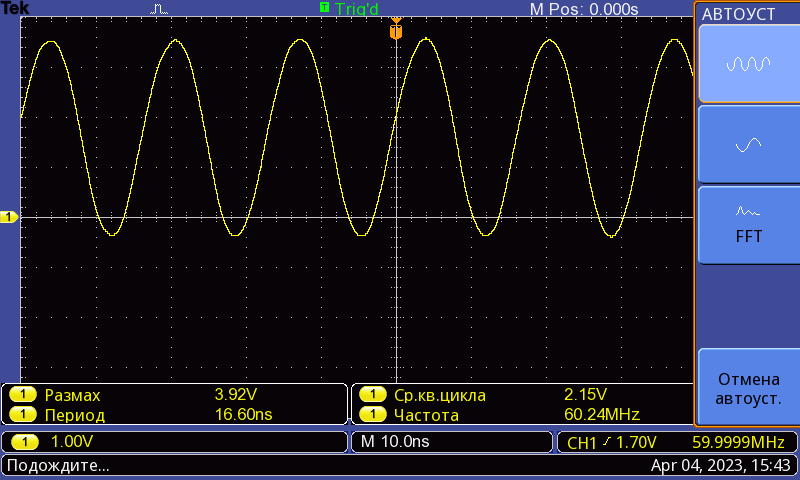
\includegraphics[width = 0.4\textwidth]{F:/git/micro/Lab5/report/sineanalog2.png}	
	\end{subfigure}
	\hfill
	\begin{subfigure}
		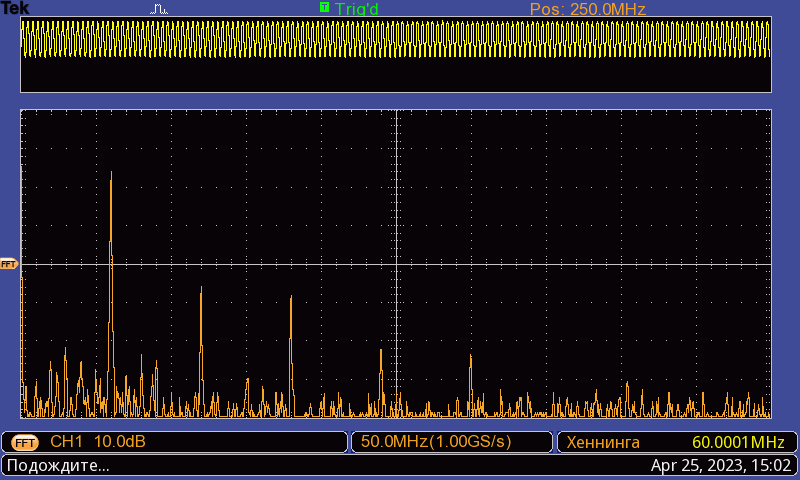
\includegraphics[width = 0.4\textwidth]{F:/git/micro/Lab5/report/FFT.png}	
	\end{subfigure}
	\caption{Синусоидальная волна}
\end{figure}



\end{document}